\documentclass[a4paper,11pt,final]{article}
% Pour une impression recto verso, utilisez plutôt ce documentclass :
%\documentclass[a4paper,11pt,twoside,final]{article}

\usepackage[english,francais]{babel}
\usepackage[utf8]{inputenc}
\usepackage[T1]{fontenc}
\usepackage[pdftex]{graphicx}
\usepackage{setspace}
\usepackage{hyperref}
\usepackage[french]{varioref}

\newcommand{\reporttitle}{Projet Yolodt}     % Titre
\newcommand{\reportauthor}{Julien \textsc{Abadji} Bastien \textsc{Lepesant}} % Auteur
\newcommand{\reportsubject}{Rapport de projet} % Sujet
\newcommand{\HRule}{\rule{\linewidth}{0.5mm}}
\setlength{\parskip}{1ex} % Espace entre les paragraphes

\hypersetup{
    pdftitle={\reporttitle},%
    pdfauthor={\reportauthor},%
    pdfsubject={\reportsubject},%
    pdfkeywords={rapport} {projet} {java} {yolodt}
}

\begin{document}
  % Inspiré de http://en.wikibooks.org/wiki/LaTeX/Title_Creation

\begin{titlepage}

\begin{center}

\begin{minipage}[t]{0.48\textwidth}
  \begin{flushleft}
    
\includegraphics [width=30mm]{images/logo-univ.jpg} \\[0.5cm]
    \begin{spacing}{1.5}
      \textsc{\LARGE Université de Cergy-Pontoise}
    \end{spacing}
  \end{flushleft}
\end{minipage}
\begin{minipage}[t]{0.48\textwidth}
  \begin{flushright}
  % 
\includegraphics [width=30mm]{images/logo-societe.jpg} \\[0.5cm]
  % \textsc{\LARGE Entreprise}%%
  \end{flushright}
\end{minipage} \\[1.5cm]

\textsc{\Large \reportsubject}\\[0.5cm]
\HRule \\[0.4cm]
{\huge \bfseries \reporttitle}\\[0.4cm]
\HRule \\[1.5cm]

\begin{minipage}[t]{0.3\textwidth}
  \begin{flushleft} \large
    \emph{Auteurs :}\\
    \reportauthor
  \end{flushleft}
\end{minipage}
\begin{minipage}[t]{0.6\textwidth}
  \begin{flushright} \large
    \emph{Jury :} \\
    M.~Marc \textsc{Lemaire} \\
    M.~Tianxiao \textsc{LIU}
  \end{flushright}
\end{minipage}

\vfill

{\large 5 Janvier 2015}

\end{center}

\end{titlepage}

  \cleardoublepage % Dans le cas du recto verso, ajoute une page blanche si besoin
  \tableofcontents % Table des matières
  \sloppy          % Justification moins stricte : des mots ne dépasseront pas des paragraphes
  \cleardoublepage
  %\include{}
  \cleardoublepage
  \section{Introduction} % Numérotation
%\addcontentsline{toc}{section}{Introduction} % Ajout dans la table des matières

\subsection{Contexte}
Nous sommes en Licence 2 Mathématiques-Informatique à l'Université de Cergy-Pontoise. Parmi les enseignements dispensés au cours du premier semestre se trouve un module de programmation orientée objet (POO), en Java. C'est dans ce contexte d'introduction à la POO que nous a été proposé le projet ( baptisé Yolodt ) dont il est question.
\subsection{Objectif}
Yolodt est un programme qui a pour objectif de proposer une indexation de fichiers de type "Open Office Document", d'un stockage de leur titres, puis d'une recherche ultérieure d'informations contenues dans ceux-ci.
\subsection{Environnement}
Le projet a été développé avec le Java Development Kit 7 (JDK 7), à l'aide de l'Environnement de Développement Integré (IDE) Eclipse Luna. 
Les systèmes d'exploitation utilisés durant toute la durée du développement ont été Debian, ArchLinux et ElementaryOS. 
Ces trois systèmes sont de type Linux.
\subsection{Composition}
Le groupe est composé de Julien Abadji et Bastien Lepesant. Nous avons des façons différentes de réfléchir, et nous avons pensé intéressant de nous mettre en binôme afin de confronter nos idées souvent divergentes, dans le but de toujours s'approcher de la conception optimale du projet.  %De plus, ceci nous a permis de mesurer l'importance de la communication dans un projet à plusieurs : en effet, sans une quasi constante remise en question des idées blahblah pour la conclusion.
  \cleardoublepage
  \section{Conception et réalisation}

\subsection{Partir de l'utilisateur pour arriver au diagramme.}

En premier lieu il nous a semblé intéressant de s'imaginer le comportement d'un utilisateur devant le programme fini. Ainsi, au fil des actions du personnage virtuel,
l'allure globale du projet se détaille.  

Le schéma d'utilisation classique part d'une importation d'un ensemble de dossiers ou fichiers de type Open Document Text ( abrégé ODT par la suite ), l'extraction d'un fichier contenant les données à analyser, l'analyse, et le stockage, ces trois dernières étapes étant totalement transparentes pour l'utilisateur.
Ensuite vient la recherche. L'utilisateur doit pouvoir entrer un ou plusieurs mots et avoir en retour une liste triée par pertinence des documents ODT les plus pertinents. 

L'étape suivante consiste à abstraire le problème en passant par un diagramme de classes UML. Après différentes discussions, le diagramme approuvé par notre groupe est celui-ci.
 \begin{figure}[!ht]
	\center
	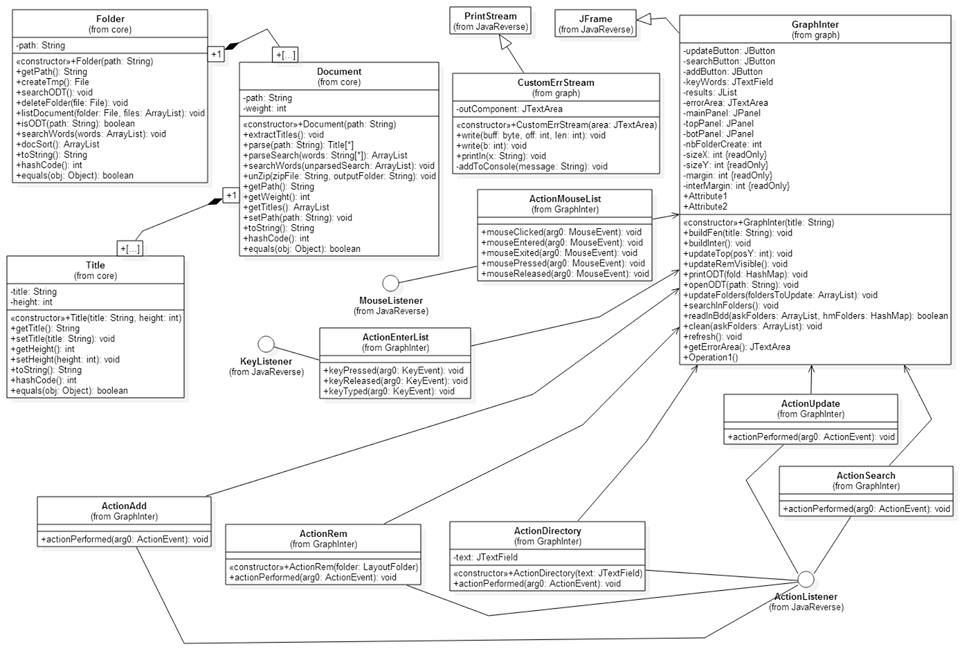
\includegraphics[width=\textwidth]{./images/uml.jpg}
	\caption{\href{http://uinelj.eu/misc/yolODT/uml.jpg}{Voir l'UML en plus grand}}
\end{figure}

\subsection{Du diagramme au code.}

Au vu de la taille du projet, la réalisation a nécessité un partage des tâches. 
Afin d'avoir une gestion du projet efficace, simple et sûre, un dépôt git\footnote{git est un logiciel de gestion de versions.} a été créé.
Ainsi, chaque modification du code est expliquée, enregistrée, et réversible en cas de problème. 

Concernant le partage des tâches suscité, Bastien s'est plus occupé des aspects d'entrée/sortie, de gestion des fichiers et de l'interface graphique, tandis que Julien
s'est focalisé sur l'extraction, l'analyse (parsage XML) et l'interface en ligne de commande. 

Le partage n'a cependant pas été hermétique : Nous nous avous mutuellement relu notre code et suggéré des améliorations. Un exemple est la gestion de la recherche. Initalement réalisée par la méthode searchWords écrite par Bastien, Julien l'a modifié légèrement et y a adjoint la méthode parseSearch, afin de proposer des possibilités de recherche plus étendues.
% On peut mettre des mots en \emph{italique}, 
% en \textsc{petites Majuscules} ou 
% en \texttt{largeur fixe (machine à écrire)}.

% Voici un deuxième paragraphe avec une formule mathématique simple : $e = mc^2$.

% Un troisième avec des \og guillemet français \fg{}.

% \subsubsection{Écrire en anglais}

% \foreignlanguage{english}{Do you speak French? Does anybody here speak french?}


% \subsection{Lites}

% \begin{itemize}
% \item Liste classique ;
% \item un élément ;
% \item et un autre élément.
% \end{itemize}
% \vspace{\parskip} % espace entre paragraphes

% \begin{enumerate}
% \item Une liste numéroté
% \item deux
% \item trois
% \end{enumerate}
% \vspace{\parskip}

% \begin{description}
% \item[Description] C'est bien pour des définitions.
% \item[Deux] Ou pour faire un liste spéciale.
% \end{description}
% \vspace{\parskip}


% \subsection{Références}

% Voici une référence à l'image de la figure \ref{bloghiko} page \pageref{bloghiko} et une autre vers la partie \ref{p2} page \pageref{p2}.

% On peut citer un livre\,\up{\cite{lpp}} et on précise les détails à la fin du rapport dans la partie références.


% \subsection{Note de bas de page}

% Voici une note\,\footnote{Texte de bas de page} de bas de page.
% Une deuxième\,\footnotemark{} déclarée différemment.
% La même note\,\footnotemark[\value{footnote}].

% \footnotetext{Il a deux références vers cette note}


% \subsection{Figure}

% \begin{figure}[!ht]
%     \center
%     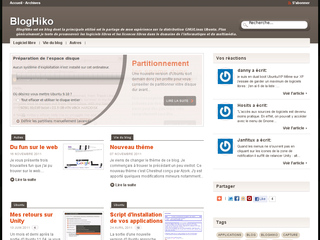
\includegraphics[width=0.5\textwidth]{./images/bloghiko.jpg}
%     \caption{BlogHiko | 50\% de la largeur de la page}
% \end{figure}



  \cleardoublepage
  \section{Manuel utilisateur}
%\label{p2}
Le programme est utilisable en deux versions : Une première non-interactive en ligne de commande, et une seconde interactive graphique.
\subsection{Interface en ligne de commande}

Le programme peut être invoqué avec 3 arguments différents. L'abscence de arguments renvoie une erreur et un rappel sur la syntaxe des arguments attendus.

-d <folder1> <folder2> ... : Ajoute les dossiers folder1 folder2 ... à la base de données, c'est-à-dire recherche récursivement tous les ODT présents dans ces dossiers, extrait et analyse leur contenu et enregistre les titres pour une recherche future.

-f <file> : Affiche les informations importantes de l'ODT file : Chemin, titres.

-w <words> : Retourne les ODT les plus pertinents en fonction des mots recherchés. Si un "+ " est envoyé, la recherche se fera en mode ET (ie. on cherchera un ODT contenant tous les mots spécifiés après le +). Si un ensemble de mots est spécifié entre guillemets, le programme ne retournera que des ODT contenant exactement la phrase entre guillemets.

\newpage
\subsection{Interface graphique}
 \begin{figure}[!ht]
	\center
	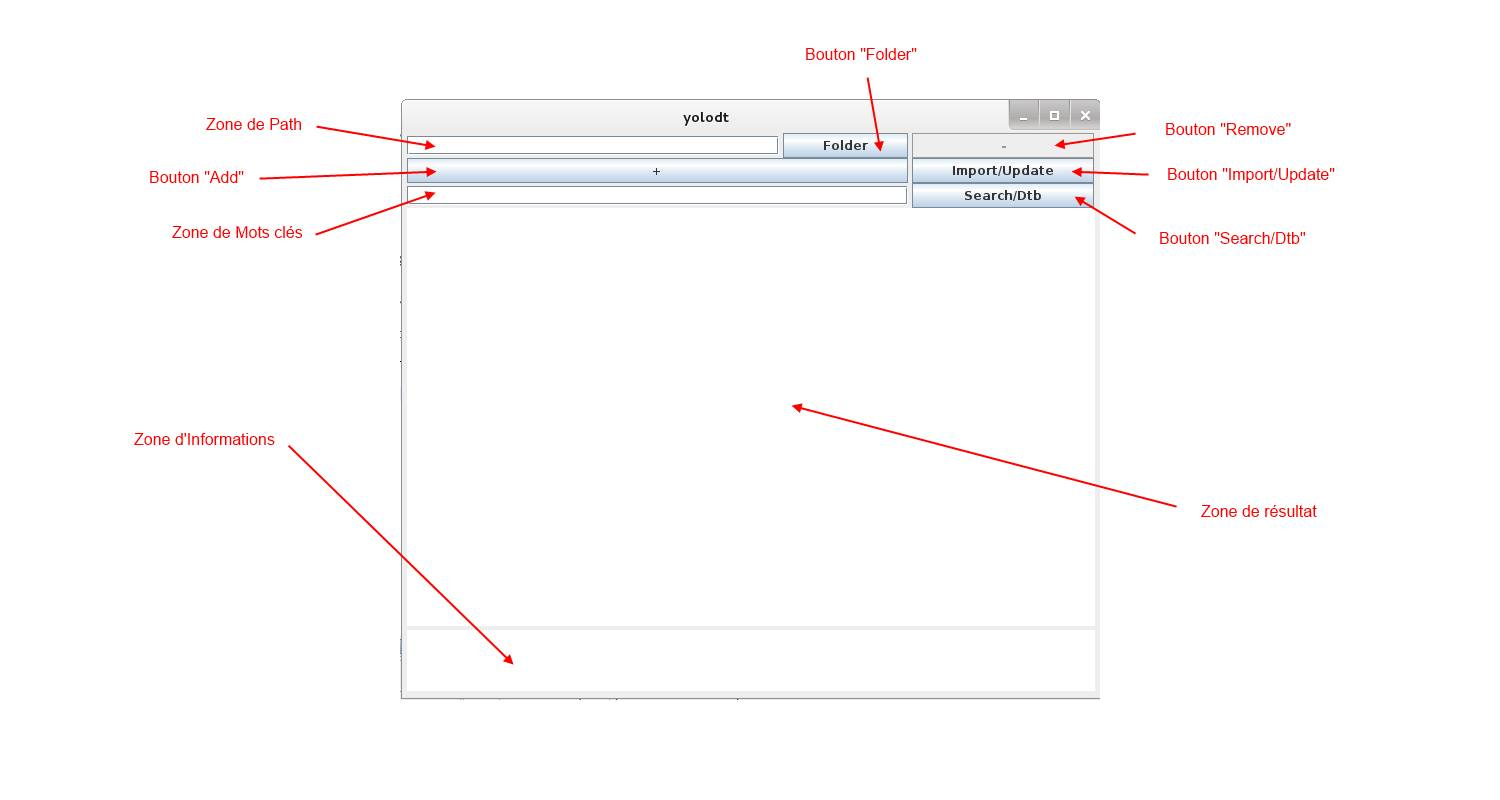
\includegraphics[width=\textwidth]{./images/gui.jpg}
\end{figure}

Résultats : L'affichage des résultats se fera dans la Zone de Résultat. 
Pour accéder a un résultat, vous pouvez double cliquer dessus au le sélectionner et appuyer sur la touche "Entrée".

Informations : L'affichage d'informations se fera dans la Zone d'Information

Zone de Path : La Zone de Path est située en haut à gauche de l'écran. Pour y ajouter plus de path, cliquer sur le bouton "Add". Pour en enlever cliquez sur le bouton "Remove". 
S'il ne reste qu'un champs, il ne peut être enlevé.

Zone de mots clés : Cette sert pour la recherche par mots clés. Mettre les mots clés recherchés séparés par un espace. Vous pouvez leurs appliquer les opérateurs suivant :
-> Si le premier mot est un "-", l'opérateur OU sera appliqué (les mots seront indépendant les uns des autres.)
Cette opérateur est utilisé par défault si le premier mot n'est ni "-", ni "+"
-> Si le premier mot est un "+", l'opérateur ET sera appliqué (le programme ne donnera que les fichiers contenant l'intégralité des mots)
-> Si plusieurs mots sont entouré par des guillemets (exemple : "Le fichier"), cela ne sera considéré que comme un unique mot

- Pour Mettre à jour la base de données :
--> Insérer les dossiers voulu dans la Zone de Path (cf Zone de Path) puis clicker sur le bouton "Import/Update"

- Pour afficher la base de données entièrement : Clicker sur le Bouton "Search/Dtb" en laissant les champs vides.

- Pour rechercher des mots dans l'intégralité de la base de données : Clicker sur le Bouton "Search/Dtb" après n'avoir rempli que la Zone de Mots Clés (cf Zone de Mots Clés)

- Pour afficher les fichiers ODT d'un ou plusieurs Path en particulier, Clicker sur le Bouton "Search/Dtb" après n'avoir remplie que la Zone de Path (cf Zone de Path)

Pour rechercher des mots dans les fichiers ODT d'un ou plusieurs Path en particulier : Clicker sur le Bouton "Search/Dtb" en ayant remplie la Zone de Path (cf Zone de Path) et la Zone de Mots Clés (cd Zone de Mots Clés)

  \cleardoublepage
  \section*{Conclusion}
\addcontentsline{toc}{section}{Conclusion}

Ce projet a été pour nous l'occasion de découvrir le travail collaboratif sur un projet concret. Nous avons constaté que cette méthode de travail avait des avantages indéniables (productivité, apports de l'argumentation et de la revue de code..), mais pouvait potentiellement être très chronophage et ralentissante sans planification des tâches et utilisation d'outils de travail collaboratifs (git). 
De plus, ce travail nous a permis de mesurer l'importance de la communication dans un projet à plusieurs : en effet, sans une quasi constante remise en question de nos idées le projet aurait pu être bien plus complexe à réaliser. 

Durant nos tests nous avons constaté un bon fonctionnement du programme. Cependant, il est coutume de dire qu'un projet n'est jamais fini.
De nombreuses améliorations sont à imaginer : Effectuer la recherche dans les paragraphes, améliorer l'interface non-graphique afin de l'adapter à une utilisation par un humain et par un script (avec des sorties en XML, JSON, etc.)...
  \cleardoublepage
  %\phantomsection\addcontentsline{toc}{section}{Références}
\begin{thebibliography}{ABC}	
    \bibitem[REF]{reference} auteur. \emph{titre}. édition, année.
    \bibitem[LPP]{lpp} Rolland. \emph{LaTeX par la pratique}. O'Reilly, 1999.
\end{thebibliography}

\end{document}

